\documentclass[a4paper]{article}
\usepackage[utf8]{inputenc}
\usepackage[T1]{fontenc}
\usepackage[polish]{babel}
\usepackage{graphicx}
\usepackage{listings}
\usepackage{float}
\usepackage{geometry}
 \geometry{
 a4paper,
 total={170mm,257mm},
 left=20mm,
 top=20mm,
 }

\graphicspath{ {./images/} }

\author{Michał Stefanik}
\date{\today}
\title{Raport z zadania 4. - Transfer Learning}

\begin{document}

\maketitle
\section{Wstęp}
Do wykonania zadania używałem języka Python 3.10.13
z biblioteką PyTorch 2.1.0.

\section{Zadanie}

Należało pobrać model yolov8, przetrenować go na zbiorze danych, oraz rozmyć wykryte obiekty na obrazkach.
Zbiór danych wygenerowano na podstawie openimages, biorąc podzbiór obrazków zawierających jedzenie.

\section{Test podstawowego modelu}

Przed rozpoczęciem treningu sprawdzono działanie podstawowego modelu na przykładowym obrazku.
Przykładowy obrazek został przedstawiony na rysunku \ref{fig:cat_dog}.
Predykcja modelu została przedstawiona na rysunku \ref{fig:cat_dog_pred}.
Model prawidłowo rozpoznał psa, wyjątkowo nie rozpoznał kota, a zamiast tego wykrył niedźwiedzia.

\begin{figure}[H]
    \centering
    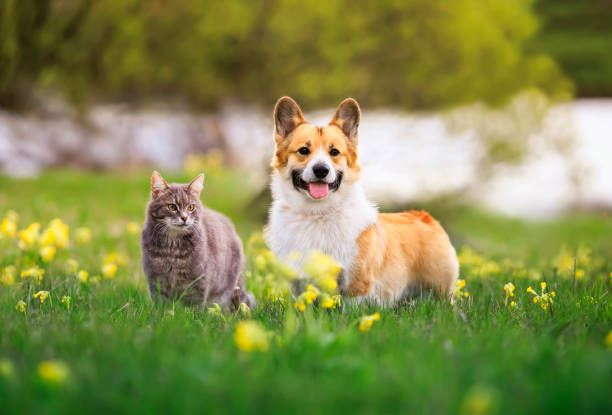
\includegraphics[width=0.5\textwidth]{cat_dog.jpg}
    \caption{Przykładowy obrazek}
    \label{fig:cat_dog}
\end{figure}

\begin{figure}[H]
    \centering
    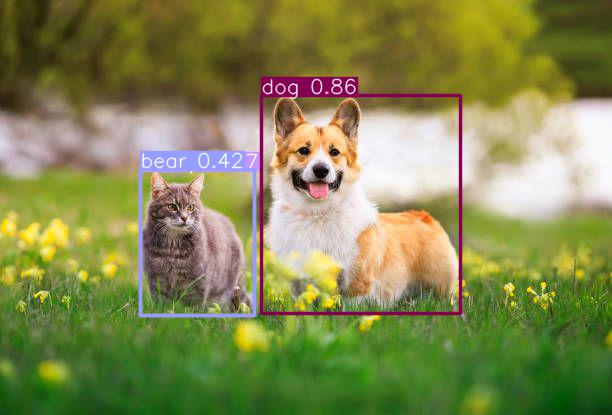
\includegraphics[width=0.5\textwidth]{cat_dog_result.jpg}
    \caption{Predykcja podstawowego modelu}
    \label{fig:cat_dog_pred}
\end{figure}

\section{Przygotowanie danych}
Większość pracy w zadaniu polegała na przygotowaniu danych do treningu. W tym celu zostały przeczytane pliki z openimages dotyczące
pudełek (oidv6-train-annotations-bbox.csv) oraz klas (oidv6-class-descriptions.csv). Następnie wybrałem 5000 obrazków oraz
odpowiadające im pudełka. Na ich podstawie wygenerowałem plik train\_download.txt oraz wpisy do datasets/train\_data. Zawierają one
informacje o klasach oraz lokalizacjach pudełek na obrazkach. Na podstawie train\_download.txt skrypt ze strony openimages pobrał
obrazki. Identyczne kroki zostały wykonane dla zbioru walidacyjnego i testowego.

\section{Trening}

Do treningu użyto modelu yolov8n.

\section{Wynik treningu}

Po 5 epokach treningu model na niektórych obrazkach prawidłowo rozpoznaje jedzenie.
Przykładowe predykcje zostały przedstawione na rysunku \ref{fig:predictions}.
Niestety, na sporej części obrazków model nie rozpoznaje jedzenia, lub zaznacza za duży obszar.
Wykryte obiekty rozmyłem używając Pythona z Pillow. Przykładowe obrazki zostały przedstawione na rysunku \ref{fig:blurred}.

\begin{figure}[H]
    \centering
    \includegraphics[width=\textwidth]{images/predictions.png}
    \caption{Przykładowe predykcje}
    \label{fig:predictions}
\end{figure}

\begin{figure}[H]
    \centering
    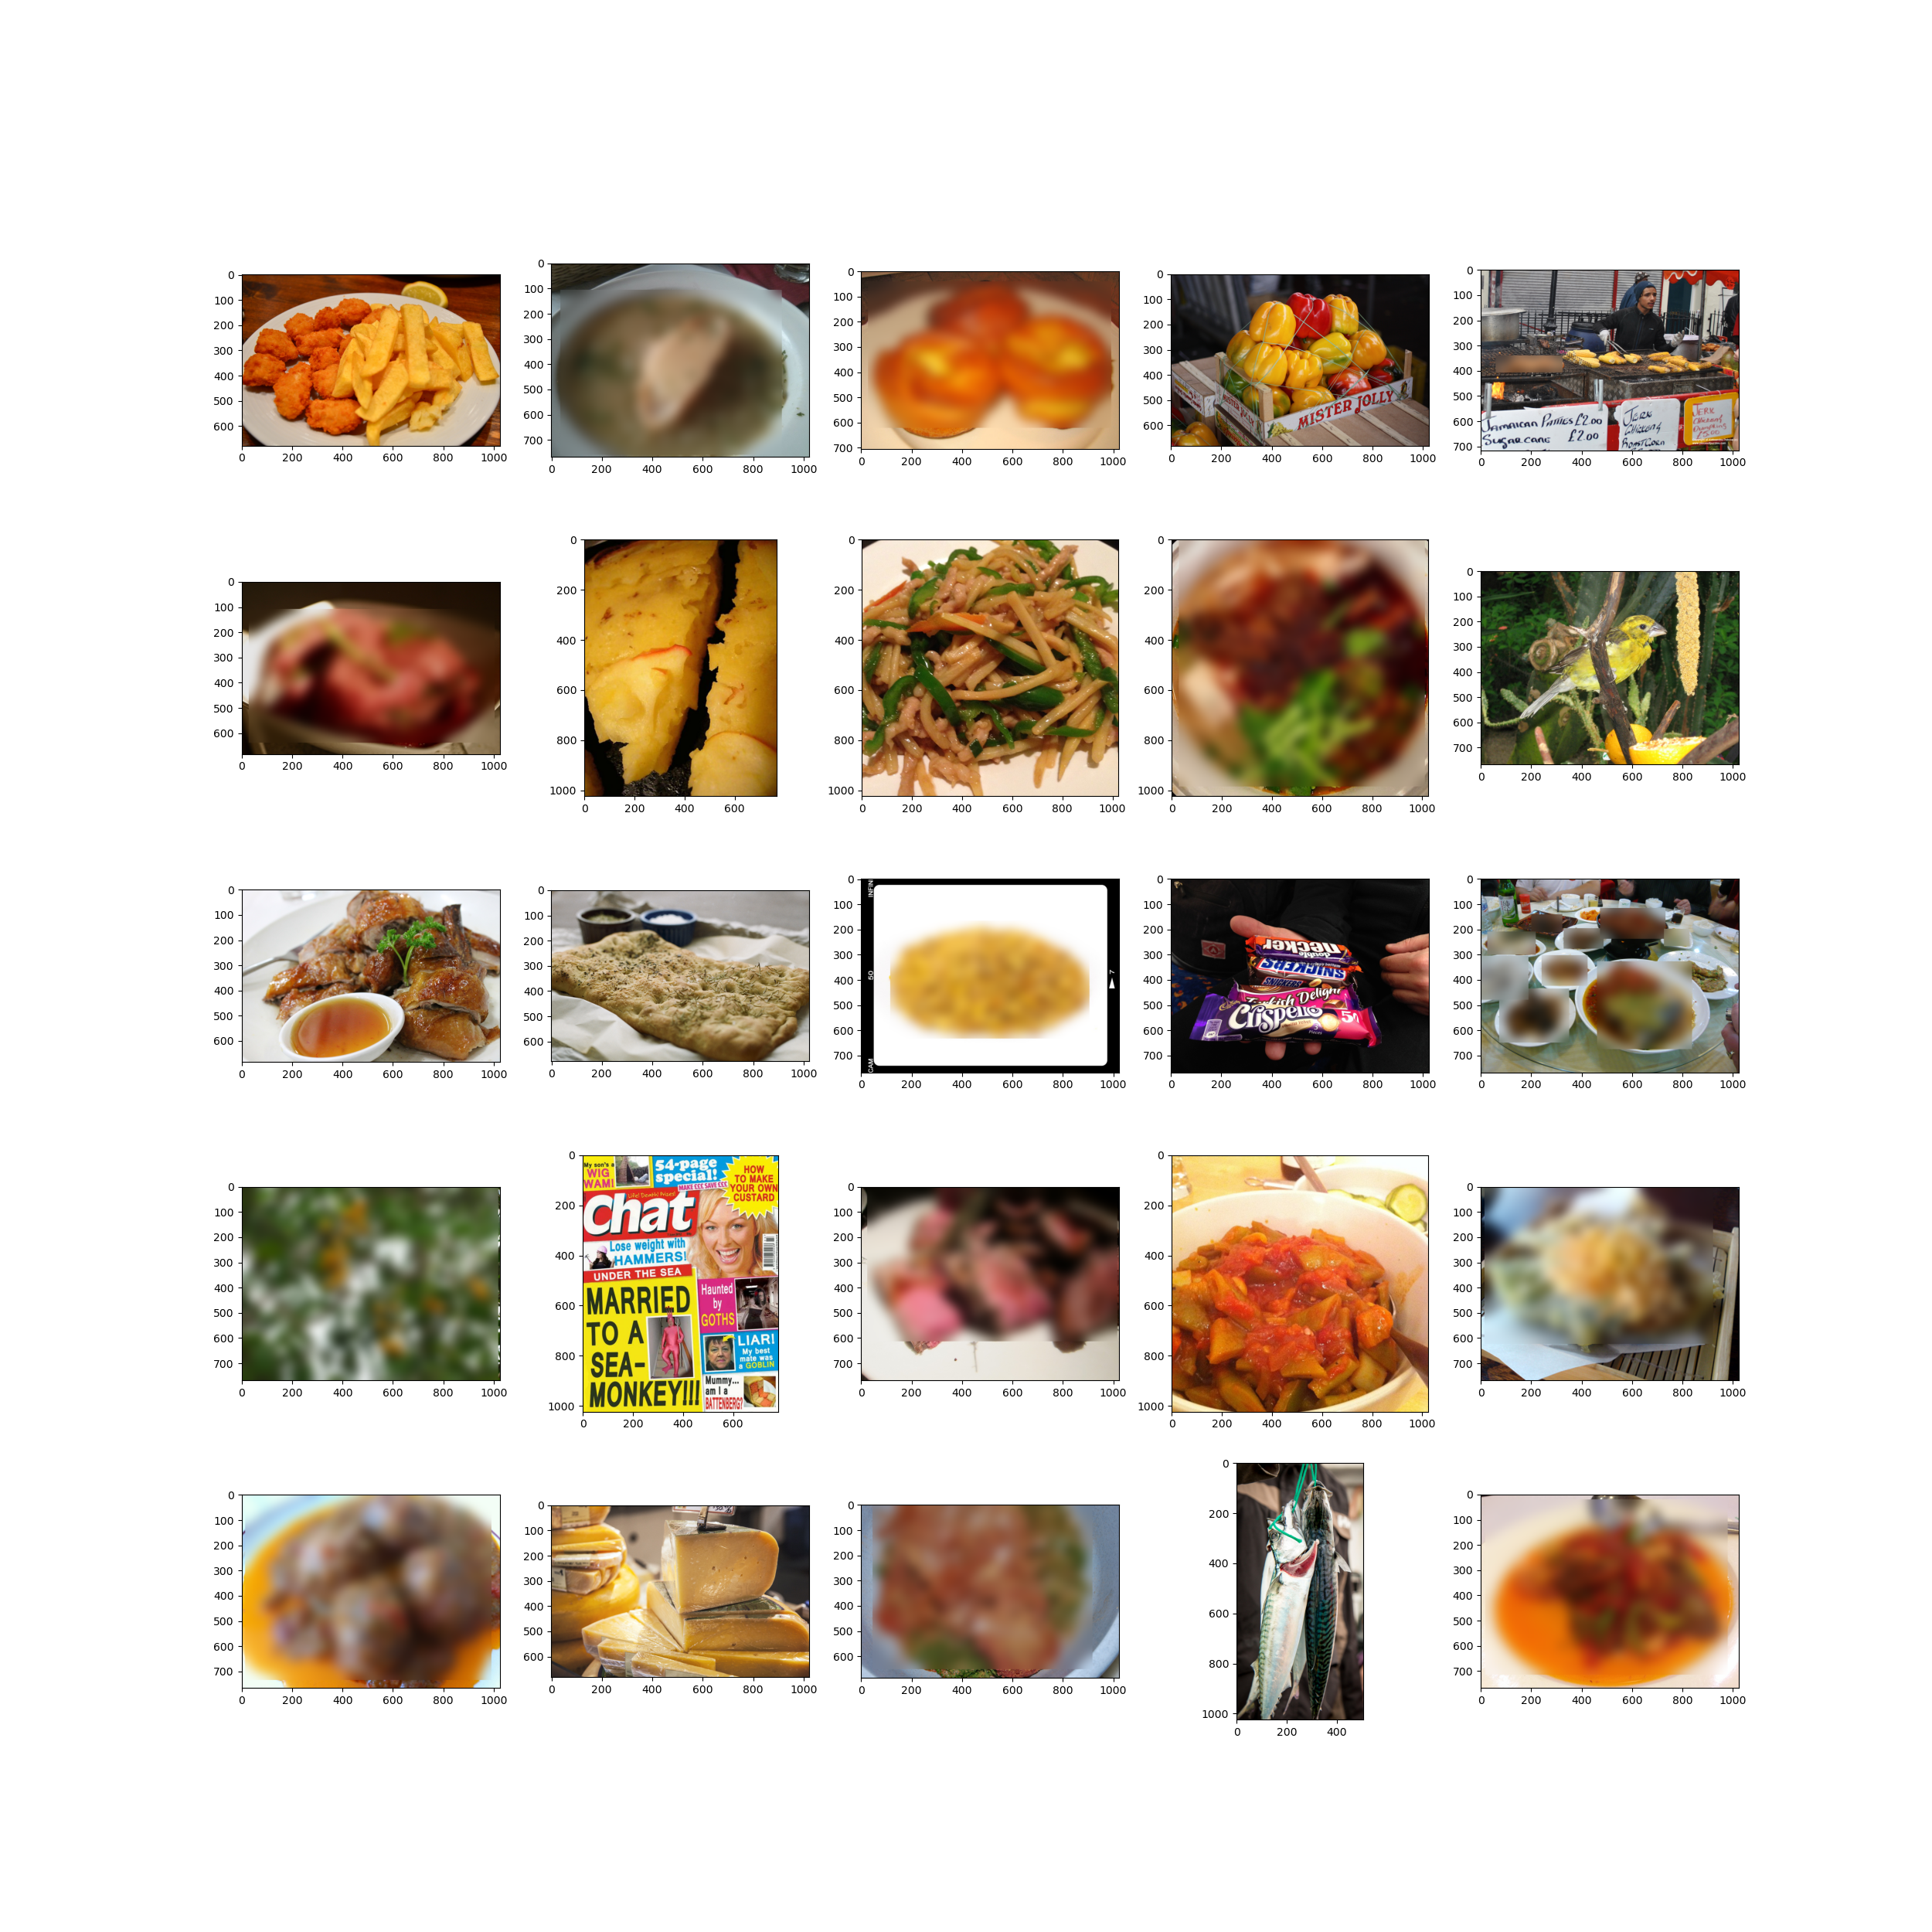
\includegraphics[width=\textwidth]{images/blurred.png}
    \caption{Ocenzurowane obrazki}
    \label{fig:blurred}
\end{figure}


\end{document}
